\documentclass{beamer}

\usepackage[utf8]{inputenc}
\usecolortheme{beaver}
\usepackage{caption}
\usepackage{subcaption}
\usepackage{mathtools}
\usepackage{todonotes}
\usepackage{amsmath}
\usepackage{bm}
\usepackage{listings}
\usepackage{ragged2e}
\usepackage{fancyvrb}
\usepackage{titlecaps}

\Addlcwords{for a is but and with of in as the etc on to if}

\def\ci{\perp\!\!\!\!\!\perp}

\tikzstyle{latent} = [ draw, circle, inner sep = 2pt, minimum size = 0.65cm ]
\tikzstyle{observed} = [ draw, rectangle, inner sep = 2pt, minimum size = 0.65cm ]

\newtheorem{proposition}{Proposition}

\setbeamertemplate{section in toc}{\inserttocsectionnumber.~\inserttocsection}
\usetheme{Boadilla}
\makeatletter
\setbeamertemplate{footline}{%
    \leavevmode%
    \hbox{%
        \begin{beamercolorbox}[wd=.3\paperwidth,ht=2.25ex,dp=1ex,center]{author in head/foot}%
            \usebeamerfont{author in head/foot}\insertshortauthor\expandafter\beamer@ifempty\expandafter{\beamer@shortinstitute}{}{~~(\insertshortinstitute)}
        \end{beamercolorbox}%
        \begin{beamercolorbox}[wd=.55\paperwidth,ht=2.25ex,dp=1ex,center]{title in head/foot}%
            \usebeamerfont{title in head/foot}\insertshorttitle
        \end{beamercolorbox}%
        \begin{beamercolorbox}[wd=.15\paperwidth,ht=2.25ex,dp=1ex,right]{date in head/foot}%
            \usebeamerfont{date in head/foot}\insertshortdate{}\hspace*{2em}
            \insertframenumber{} / \inserttotalframenumber\hspace*{2ex} 
        \end{beamercolorbox}}%
        \vskip0pt%
    }
\makeatother

\begin{document}

\title[]{Validating Causal Inference Methods}
\author [] {}
\date{}

\begin{frame}
	\frametitle{Motivation}
	\begin{itemize}
		\item Many statistical methods for causal inference under unconfoundedness conditions.
		\item Examples are propensity score based methods, prognostic score-based methods, and doubly robust methods.
		\item Most of these methods are evaluated on simulated datasets which are not the reality.
		\item Crucial to understand how these methods perform on the data at hand.
	\end{itemize}
	\begin{figure}
		\includegraphics{imgs/comparison.png}
	\end{figure}
\end{frame}
\begin{frame}
	\begin{itemize}
		\item The performance of these methods is fairly well understood and if they can be estimated at sufficiently fast rates, they perform well.
		\item But if any finite sample size, the performance of these methods vary significantly.
		\item Details on the problems with each of these methods in section Causal effect estimation section.
		\item Existing approaches: 
			\begin{itemize}
				\item Face validity test: Compares the estimated treatment effect against an expert's intuition.
				\item Placebo or negative control: In-time placebo: restricts the analysis to a time period where the effect is known to be null. In-sample: control unit should have zero effect.
				\item Synthetic data sets: A data generating mechanism that gives access to true causal effects.
			\end{itemize}
	\end{itemize}
\end{frame}

\begin{frame}
	\frametitle{The proposed framework}
	\begin{itemize}
		\item A deep generative framework to evaluate causal inference methods.
		\item Allows users to specify the ground truth for the form and magnitute of causal effects and confounding bias as functions of covariates.
		\item A general framework (Credence) to validate and evaluate existing causal inference methods using synthetic data anchored at the empirical distribution of a given dataset.
		\item Two important properties: 1) User-specified causal treatment effects, heterogeneity, and endogeneity. 2) simulated samples that are stochastically indistinguishable from the observed data sample of interest.
		\item Trained on a rich universe of data sets that share certain key features.
	\end{itemize}
\end{frame}

\begin{frame}
	\frametitle{Framework}
	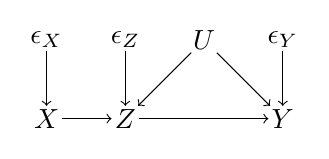
\begin{tikzpicture}	
		\tikzstyle{every node}=[align=center, inner sep=1pt]
		\node (x) at (0, 0) {$ X $};
		\node (epsx) at (0, 1) {$ \epsilon_X $};
		\node (z) at (1, 0) {$ Z $};
		\node (epsz) at (1, 1) {$ \epsilon_Z $};
		\node (u) at (2, 1) {$ U $};
		\node (y) at (3, 0) {$ Y $};
		\node (epsy) at (3, 1) {$ \epsilon_Y $};

		\draw [->] (epsx) -- (x);
		\draw [->] (x) -- (z);
		\draw [->] (epsz) -- (z);
		\draw [->] (u) -- (z);
		\draw [->] (epsy) -- (y);
		\draw [->] (z) -- (y);
		\draw [->] (u) -- (y);
	\end{tikzpicture}
	$$ f(x) = \mathbb{E}[Y(1) - Y(0)| X=x] $$
	$$ g(x, z) = \mathbb{E}[Y(z) | X=x, Z=z] - \mathbb{E}[Y(z) | X=x, Z=1-z ] $$
	Minimizing:
\begin{equation}
	\begin{split}
	\textit{min}_{\theta} & \mathbb{E}[d((X, Y, Z) - (X', Y', Z'))] + \\
			& \alpha \mid\mid \mathbb{E}[Y'(1) - Y'(0) | X'=x'] - f(x') \mid\mid \\
			& \beta \mid\mid \mid\mid
\end{split}
\end{equation}
\end{frame}

\begin{frame}
	\frametitle{Discussion Points}
	\begin{itemize}
		\item There can be multiple DAGs which would generate the same observational dataset. How realistic is the assumption that the causal estimate generated from this is the true one.
		\item Why is assumption 2 needed? Shouldn't it be automated and the user shouldn't need to specify that?
	\end{itemize}
\end{frame}
\end{document}
